\documentclass[tikz,border=5pt]{standalone}
% Shared visual grammar: role fills, dark connectors, and 7-point typography.
% Build each standalone figure from this directory. No external images required.
\pdfinfoomitdate=1
\pdftrailerid{}
\usepackage[T1]{fontenc}
\usepackage{helvet}
\renewcommand{\familydefault}{\sfdefault}
\usepackage{amsmath,amssymb}
\hyphenpenalty=10000
\exhyphenpenalty=10000
\usetikzlibrary{arrows.meta,calc,fit,positioning,decorations.pathreplacing,backgrounds}
\definecolor{ink}{HTML}{172B3A}
\definecolor{muted}{HTML}{586D85}
\definecolor{datafill}{HTML}{F1F5F9}
\definecolor{dataline}{HTML}{62748E}
\definecolor{modelfill}{HTML}{E5E9FF}
\definecolor{modelline}{HTML}{7887C7}
\definecolor{llmfill}{HTML}{FFE4E8}
\definecolor{llmline}{HTML}{E68494}
\definecolor{truthfill}{HTML}{D0FAE5}
\definecolor{truthline}{HTML}{35A782}
\newcommand{\seven}{\fontsize{7}{8.5}\selectfont}
\tikzset{
 every node/.append style={font=\seven,text=ink,align=center},
 box/.style={draw=dataline,fill=white,rounded corners=3pt,line width=.65pt,inner sep=5pt,minimum height=8mm},
 data/.style={box,fill=datafill},
 model/.style={box,draw=modelline,fill=modelfill},
 llm/.style={box,draw=llmline,fill=llmfill},
 truth/.style={box,draw=truthline,fill=truthfill},
 title/.style={font=\seven\bfseries,inner sep=1pt},
 word/.style={text=muted,inner sep=1pt,align=center},
 label/.style={fill=white,inner xsep=2pt,inner ysep=1pt,text=muted},
 flow/.style={-{Stealth[length=2.4mm,width=1.9mm]},draw=ink,line width=1.2pt,shorten >=1.5pt},
 branch/.style={-{Stealth[length=2mm,width=1.6mm]},draw=ink,line width=.9pt,shorten >=1pt},
 route/.style={draw=ink,line width=1.2pt},
 update/.style={-{Stealth[length=2.2mm,width=1.7mm]},draw=modelline,line width=1pt,dash pattern=on 3pt off 2pt,shorten >=1.5pt},
 boundary/.style={draw=dataline,dash pattern=on 3pt off 2pt,rounded corners=3pt,line width=.6pt},
 chip/.style={minimum height=4mm,inner xsep=3pt,inner ysep=1.5pt,rounded corners=2pt},
}
% Optional role key. Anchor at the center of an uncluttered final row.
\newcommand{\rolekey}[2]{
 \node[word,anchor=east] at (#1-6.6,#2) {\textit{Key}};
 \node[data,chip] at (#1-5.2,#2) {records / data};
 \node[model,chip] at (#1-1.9,#2) {learned model / policy};
 \node[llm,chip] at (#1+1.65,#2) {LLM signal};
 \node[truth,chip] at (#1+4.95,#2) {labels / evaluation};
}

\newcommand{\examplefont}{\fontsize{9}{11}\selectfont}
\definecolor{negativefill}{HTML}{FFF2D8}
\begin{document}
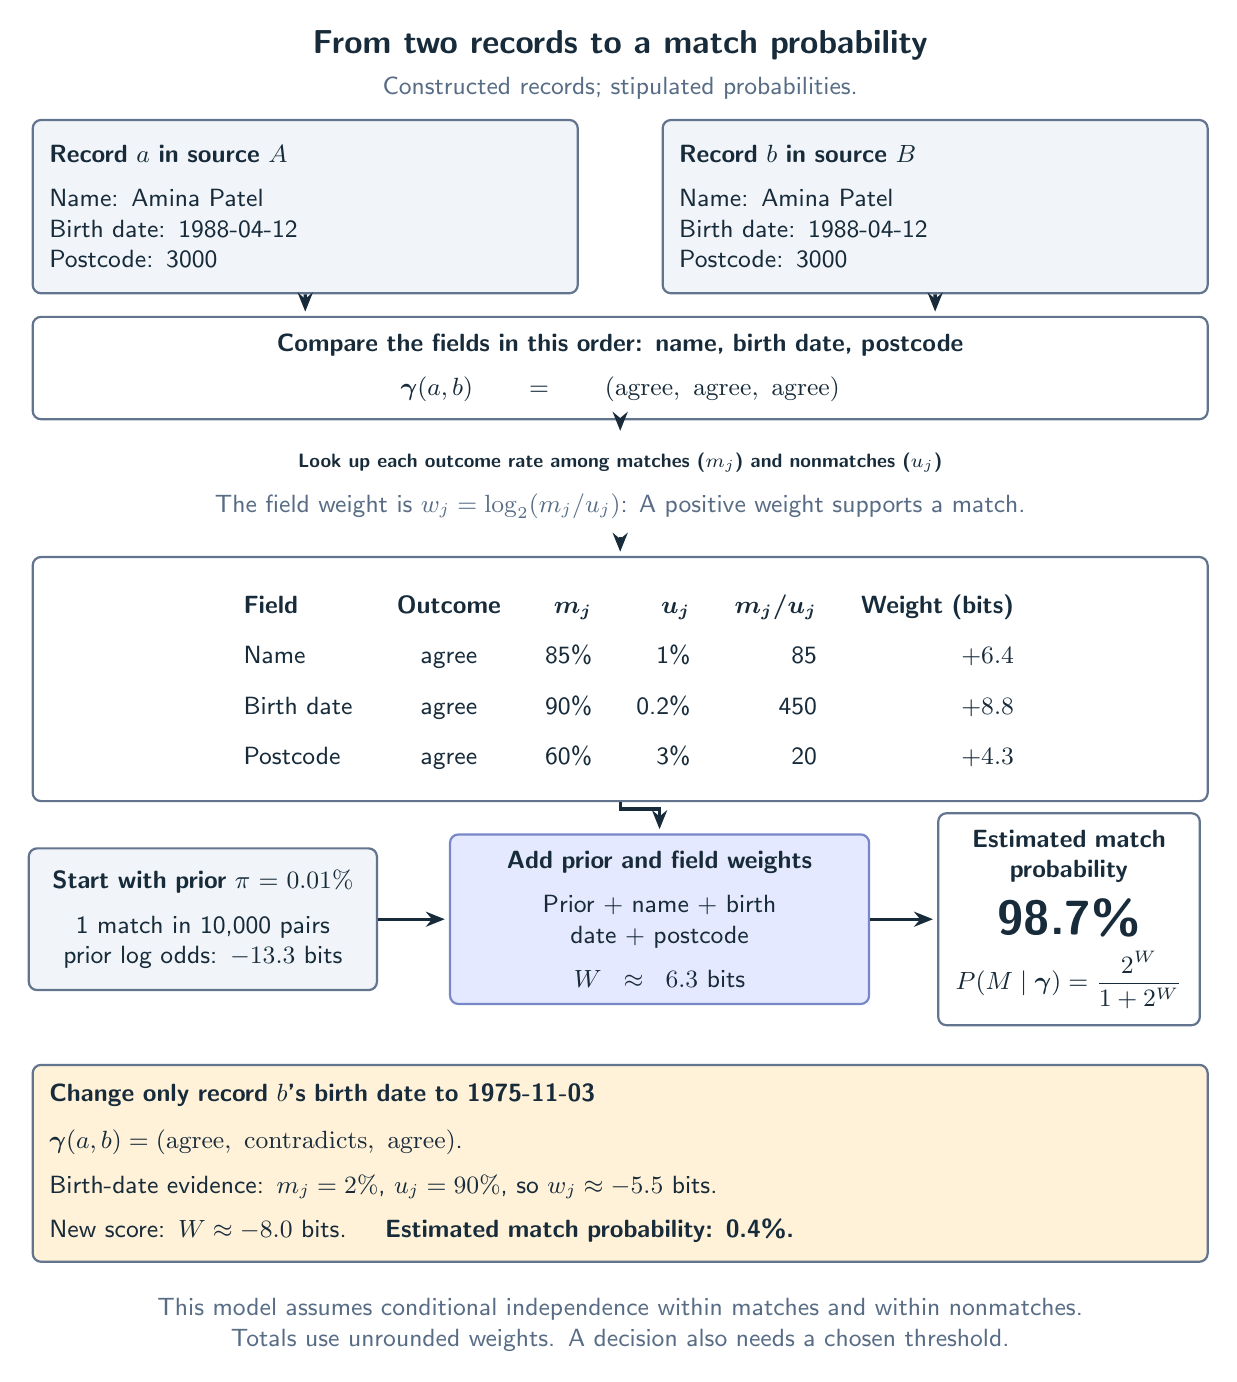
\begin{tikzpicture}[every node/.append style={font=\examplefont},
  box/.append style={inner sep=6pt,line width=.8pt}]

\node[title,font=\fontsize{12}{14}\selectfont\bfseries] at (8,0) {From two records to a match probability};
\node[word] at (8,-.55) {Constructed records; stipulated probabilities.};

\node[data,text width=65mm,minimum height=22mm,align=left] (a) at (4,-2.05) {
  \textbf{Record $a$ in source $A$}\\[5pt]
  Name: Amina Patel\\
  Birth date: 1988-04-12\\
  Postcode: 3000};
\node[data,text width=65mm,minimum height=22mm,align=left] (b) at (12,-2.05) {
  \textbf{Record $b$ in source $B$}\\[5pt]
  Name: Amina Patel\\
  Birth date: 1988-04-12\\
  Postcode: 3000};

\node[box,text width=145mm,minimum height=13mm] (gamma) at (8,-4.1) {
  \textbf{Compare the fields in this order: name, birth date, postcode}\\[5pt]
  $\boldsymbol\gamma(a,b)=(\mathrm{agree},\ \mathrm{agree},\ \mathrm{agree})$};
\draw[flow] (a.south) -- ([xshift=-40mm]gamma.north);
\draw[flow] (b.south) -- ([xshift=40mm]gamma.north);

\node[title] at (8,-5.3) {Look up each outcome rate among matches ($m_j$) and nonmatches ($u_j$)};
\node[word] at (8,-5.85) {The field weight is $w_j=\log_2(m_j/u_j)$: A positive weight supports a match.};

\node[box,text width=145mm,minimum height=31mm] (evidence) at (8,-8.05) {
  \setlength{\tabcolsep}{8pt}
  \renewcommand{\arraystretch}{1.65}
  \begin{tabular}{@{}lcrrrr@{}}
  \textbf{Field} & \textbf{Outcome} & $\boldsymbol{m_j}$ & $\boldsymbol{u_j}$ & $\boldsymbol{m_j/u_j}$ & \textbf{Weight (bits)}\\
  Name & agree & 85\% & 1\% & 85 & $+6.4$\\
  Birth date & agree & 90\% & 0.2\% & 450 & $+8.8$\\
  Postcode & agree & 60\% & 3\% & 20 & $+4.3$
  \end{tabular}};
\draw[flow] (gamma.south) -- (8,-4.95);
\draw[flow] (8,-6.25) -- (evidence.north);

\node[data,text width=40mm,minimum height=18mm] (prior) at (2.7,-11.1) {
  \textbf{Start with prior $\pi=0.01\%$}\\[5pt]
  1 match in 10,000 pairs\\
  prior log odds: $-13.3$ bits};
\node[model,text width=49mm,minimum height=18mm] (total) at (8.5,-11.1) {
  \textbf{Add prior and field weights}\\[5pt]
  Prior + name + birth date + postcode\\[5pt]
  $W\approx6.3$ bits};
\node[box,text width=29mm,minimum height=18mm] (probability) at (13.7,-11.1) {
  \textbf{Estimated match\\probability}\\[5pt]
  {\fontsize{18}{20}\selectfont\bfseries 98.7\%}\\[4pt]
  $P(M\mid\boldsymbol\gamma)=\dfrac{2^W}{1+2^W}$};
\draw[flow] (prior) -- (total);
\draw[flow] (total) -- (probability);
\draw[flow] (evidence.south) -- (8,-9.7) -| (total.north);

\node[box,fill=negativefill,text width=145mm,minimum height=25mm,align=left] (contrast) at (8,-14.2) {
  \textbf{Change only record $b$'s birth date to 1975-11-03}\\[6pt]
  $\boldsymbol\gamma(a,b)=(\mathrm{agree},\ \mathrm{contradicts},\ \mathrm{agree})$.\\[5pt]
  Birth-date evidence: $m_j=2\%$, $u_j=90\%$, so $w_j\approx-5.5$ bits.\\[5pt]
  New score: $W\approx-8.0$ bits.
  \quad\textbf{Estimated match probability: 0.4\%.}};
\node[word,text width=148mm] at (8,-16.25) {This model assumes conditional independence within matches and within nonmatches.\\Totals use unrounded weights. A decision also needs a chosen threshold.};

\end{tikzpicture}
\end{document}
